\section{Clustering}\label{sec:m2}
\attr{sp\_id} and \attr{seller\_rating\_class} never enter the clustering; the target is only used afterwards as an external label.

\subsection{Attributes and preprocessing}\label{sec:m2attr}
We cluster seven attributes that describe \emph{how a seller does business}: size (\attr{n\_listings}), market segment (\attr{price}), discounting (\attr{savings\_amount}), turnover (\attr{daysonmarket}), wear (\attr{mileage}), composition (\attr{pct\_is\_new}) and activity period (\attr{listing\_span}). The first four are log-transformed, all are standardized, and the single missing mileage is median-imputed.

The other attributes are left out on purpose and used for profiling. Vehicle specifications describe the cars and not the business, and their mutual correlation would let them dominate the distance as a block. Zero-inflated shares become artificial outliers once standardized. Mixing one-hot categoricals with continuous attributes would require an arbitrary weight. \Cref{tab:sens} supports the choice: with all 19 attributes the silhouette never exceeds 0.22 (distance concentration), and three extra specifications already lower it at every $k$. The raw scale sometimes scores higher, but by isolating extremes (at $k=3$ a group of 739 sellers), so the log view is kept.

\begin{table}[t]
\centering
\caption{K-Means silhouette by attribute set and scale (min$_4$: smallest cluster at $k=4$). The row used is the first one.}\label{tab:sens}
\tab{m2_sens}
\end{table}

\subsection{Centroid-based clustering}\label{sec:kmeans}
\paragraph{Choice of $k$} We ran K-Means for $k=2,\dots,12$ (\code{n\_init}$=10$, k-means++) and Bisecting K-Means (splitting the largest cluster), recording SSE, silhouette and Davies--Bouldin (\cref{fig:ksweep}). $k=2$ has the best silhouette (0.42) but only separates new-car from used-car sellers, which \attr{new\_used\_profile} already states (ARI 0.83). Among $k>2$, $k=4$ is the best on \emph{both} silhouette (0.343) and Davies--Bouldin (1.17); the SSE flattens after it, the smallest cluster still holds 9\% of the sellers, and from $k=6$ the silhouette falls below 0.25. Bisecting K-Means equals K-Means at $k=2$ and is worse afterwards (silhouette 0.26 at $k=4$): its greedy splits cannot be revised.

\begin{figure*}[t]
\centering
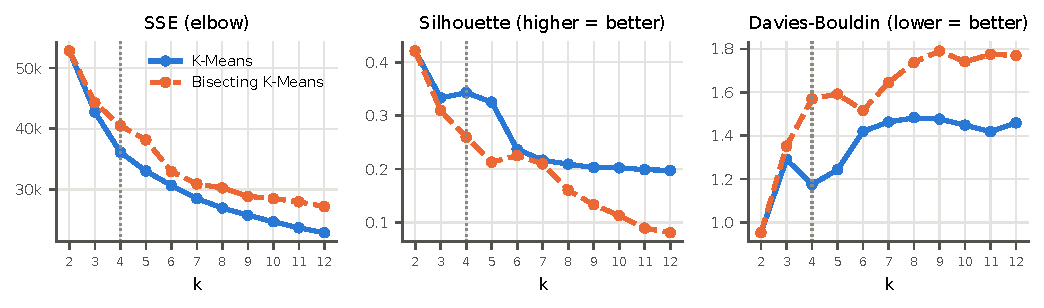
\includegraphics[width=0.95\textwidth]{m2_kmeans_sweep}
\caption{K-Means and Bisecting K-Means for $k=2,\dots,12$. Dotted line: chosen $k=4$.}\label{fig:ksweep}
\end{figure*}

\paragraph{Null model and stability} A silhouette of 0.34 is hard to judge alone, so we compared it with a null model: 20 datasets with each column permuted independently (same marginals, no dependence) and clustered in the same way (\cref{fig:validity}). The null silhouette is $0.14$--$0.16$ at every $k$ and never exceeds 0.165, so the structure is real for all $k$; but its margin falls from 0.20 at $k=4$ to 0.07 at $k=8$, and SSE relative to the null stops improving after $k=4$ (0.63, 0.56, \textbf{0.51}, 0.50, 0.49). As a second check we clustered pairs of 80\% subsamples and compared the labels of the common sellers (20 pairs per $k$): ARI is $\geq 0.99$ for $k\leq4$, then becomes unstable ($0.97\pm0.07$ at $k=5$, $0.90\pm0.15$ at $k=6$). Both checks point to $k=4$ as the finest reproducible partition.

\begin{figure*}[t]
\centering
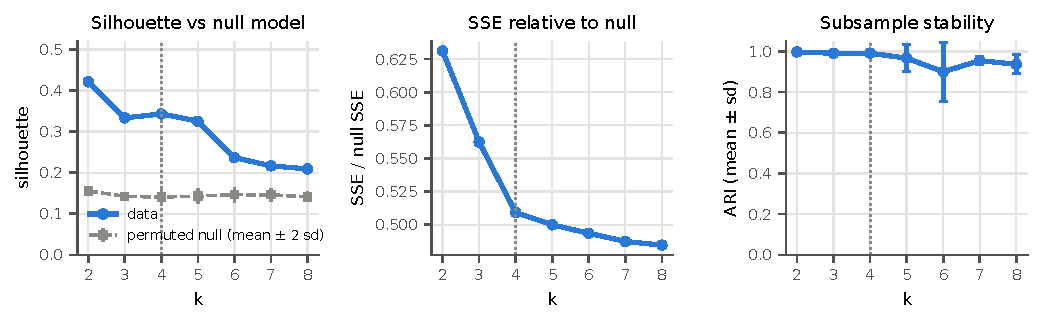
\includegraphics[width=0.95\textwidth]{m5_cluster_validity}
\caption{Cluster validity of K-Means: silhouette against 20 column-permuted null datasets, SSE relative to the null, and ARI between clusterings of random 80\% subsamples.}\label{fig:validity}
\end{figure*}

\paragraph{X-Means} We also implemented X-Means, which splits a cluster when the BIC of two spherical Gaussians beats one. It never stops on its own: $k$ grows 2, 4, 8, 15, 27, 41, 57 and reaches our cap of 64 with 20 splits still accepted. With almost 14\,000 sellers the BIC penalty is negligible against any departure from a spherical Gaussian. This is an informative negative result: the data are a continuum that can be refined indefinitely, so an automatic criterion does not replace the analysis above.

\paragraph{Profiles} \Cref{tab:prof,fig:kprof} describe the four segments, numbered by decreasing price:
\begin{itemize}
\item \textbf{C0 -- franchise new-car dealers} (37\%): large, almost zero mileage, 65\% new cars, high price, no advertised savings.
\item \textbf{C1 -- mid-market used dealers} (26\%): late-model cars ($\approx$33k miles), regular discounting; half franchise, half independent.
\item \textbf{C2 -- slow-turnover dealers} (9\%): old stock listed for 92 days against 32--39 elsewhere, over a long activity span.
\item \textbf{C3 -- small budget independents} (28\%): few listings, $\approx$113k miles, the lowest prices.
\end{itemize}
\Cref{fig:kscatter} shows that the segments occupy contiguous regions with blurred borders, not separate clouds. The rating is spread over all of them (ARI 0.014), yet the share of \emph{high} grows from 20\% in C0 to 34--36\% in C2 and C3.

\begin{table}[t]
\centering
\caption{K-Means $k=4$: cluster medians in original units (top), composition and rating mix (bottom).}\label{tab:prof}
\tab{m2_profiles}
\end{table}

\begin{figure*}[t]
\centering
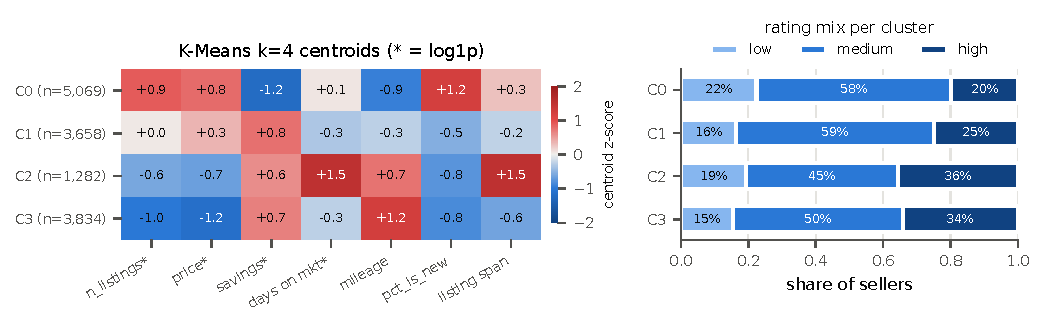
\includegraphics[width=0.95\textwidth]{m2_kmeans4_profile}
\caption{K-Means $k=4$: standardized centroids (left; * = log scale) and rating mix per segment (right).}\label{fig:kprof}
\end{figure*}

\begin{figure*}[t]
\centering
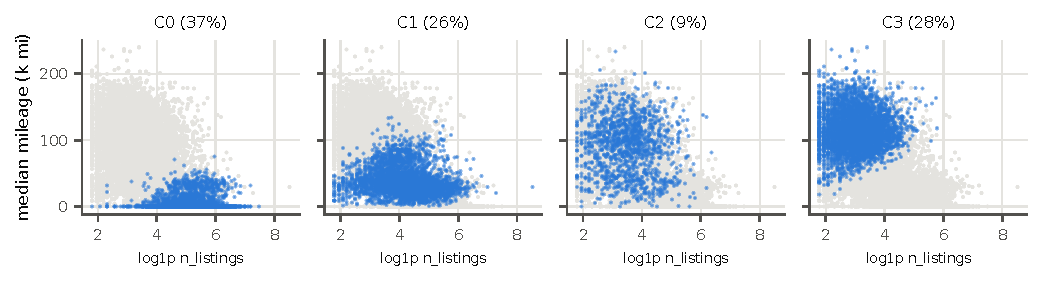
\includegraphics[width=0.93\textwidth]{m2_kmeans4_scatter}
\caption{Each K-Means segment highlighted over all sellers, in two original dimensions (size and mileage).}\label{fig:kscatter}
\end{figure*}

\subsection{Density-based clustering}\label{sec:dbscan}
\paragraph{Parameters} We kept the seven attributes: more dimensions would concentrate distances and make one global $\eps$ even harder to set. The heuristic MinPts $\approx 2d=14$ suggests the range $\{5,10,15,20,30\}$. The $k$-distance graphs (\cref{fig:kdist}) rise smoothly, without a sharp knee, between 0.35 and 1.0, which is our range for $\eps$. \Cref{tab:dbscan} reports all 45 configurations. Values at the classical knee ($\eps\geq0.7$) merge everything into one cluster; small values produce many micro-clusters and up to 87\% noise.

\begin{figure}[t]
\centering
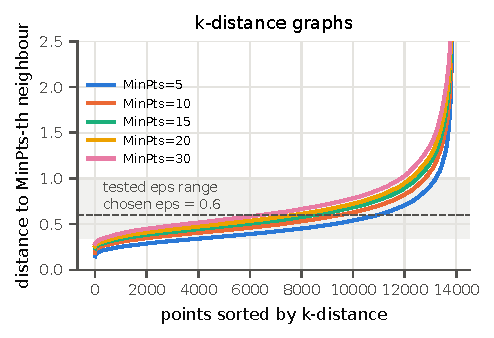
\includegraphics[width=0.94\linewidth]{m2_kdistance}
\caption{$k$-distance graphs on the seven standardized attributes, with the tested and the chosen $\eps$.}\label{fig:kdist}
\end{figure}

\begin{table*}[t]
\centering
\caption{DBSCAN, all tested configurations. Each cell: number of clusters (of which with $\geq1\%$ of the sellers); noise; silhouette on non-noise points (--: one cluster).}\label{tab:dbscan}
\tabwide{m2_dbscan}
\end{table*}

The silhouette alone would reward discarding points (0.69 with 87\% noise), so we selected, among the configurations with at least two clusters of $\geq1\%$ of the sellers, the one with the \textbf{lowest noise}: $\eps=0.6$, MinPts $=15$, with two clusters, 22\% noise and silhouette 0.49 on the retained points.

\paragraph{Result} The two dense cores are used-car dealers (D0, 6\,542, mostly C1 and C3) and franchise new-car dealers (D1, 4\,256, all from C0): the K-Means $k=2$ split. D0 has a median of 37 listings, 79k miles and \$15.2k, with 24\% franchises; D1 has 193 listings, 11 miles and \$29.8k, with 66\% new cars and only franchises. The share of \emph{high} is 29\% in D0, 19\% in D1 and 33\% in the noise. \Cref{tab:noise} characterizes the 3\,045 noise sellers: they are not corrupted records. Slow turnover dominates (a median above 120 days on market is 76 times more frequent than in the cores; 77\% of C2 is noise), followed by extreme prices and tiny inventories (ratio 3--4). Large sellers are not over-represented.

\begin{table}[t]
\centering
\caption{Traits of DBSCAN noise vs core sellers.}\label{tab:noise}
\tab{m2_noise}
\end{table}

\paragraph{OPTICS} The reachability plot (\cref{fig:optics}, MinPts $=15$) shows two broad valleys, the two cores, separated by a short rise, and then a steady climb through the noise. Cutting it at 0.6 reproduces DBSCAN (ARI 0.999), while the $\xi$ method ($\xi=0.05$), which needs steep walls, returns a single cluster. Density varies continuously, so a density-based method has no natural threshold here.

\begin{figure}[t]
\centering
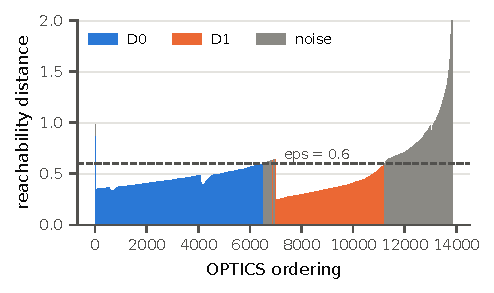
\includegraphics[width=0.94\linewidth]{m2_optics_reachability}
\caption{OPTICS reachability plot, coloured by DBSCAN label.}\label{fig:optics}
\end{figure}

\subsection{Sensitivity of K-Means to outliers}\label{sec:m2core}
We refitted K-Means ($k=4$) on the DBSCAN core points and assigned all sellers to the new centroids: ARI 0.79 with the original partition. C0 and C1 survive unchanged; C2 disappears, because its members are mostly noise, and the freed centroid splits C3. C2 is therefore a real but \emph{sparse} segment, defined by its tail behaviour. We keep it for its business meaning and report this caveat.

\subsection{Hierarchical clustering}
We clustered all 13\,843 sellers with seven linkage/distance pairs: Single, Complete, Average and Ward with Euclidean distance (Ward minimizes the within-cluster variance increase and is defined only for it), Complete and Average with Manhattan (less sensitive to one large difference), and Average with cosine (profile shape, ignoring magnitude). \Cref{fig:dendro} shows six dendrograms, \cref{tab:hier} the cophenetic correlation $r_c$ and the silhouette of the cuts (computed with the same distance).

\begin{figure*}[t]
\centering
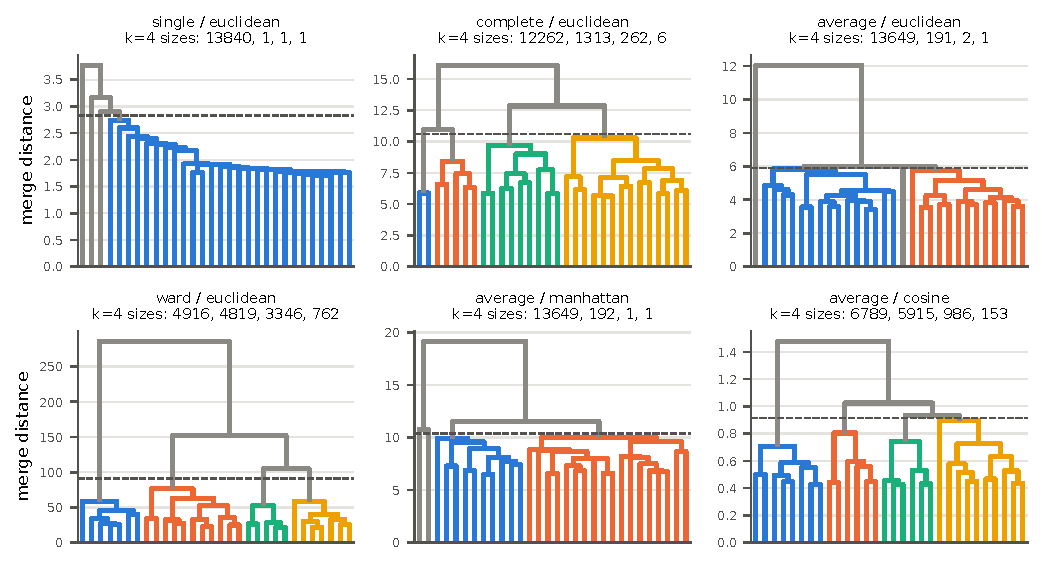
\includegraphics[width=0.95\textwidth]{m2_dendrograms}
\caption{Dendrograms (last 30 merges). Dashed line: height that gives four clusters, whose sizes are in the titles.}\label{fig:dendro}
\end{figure*}

\begin{table}[t]
\centering
\caption{Hierarchical clustering: cophenetic correlation, silhouette of the cuts $k=2,\dots,6$, and extreme cluster sizes at $k=4$.}\label{tab:hier}
\tabtight{m2_hier}
\end{table}

\textbf{Single} linkage chains: its $k=4$ cut is one giant cluster plus three singletons, and its silhouette (0.53) is an artefact of isolating outliers. \textbf{Average} (Euclidean and Manhattan) has the same defect in milder form. \textbf{Complete} is driven by maximum distances: 89\% of the sellers fall in one cluster. \textbf{Cosine/Average} has the best $r_c$ (0.86) and a balanced $k=2$ cut, but it ignores how far a seller is from the mean profile and adds a 153-seller fringe. \textbf{Ward} gives compact, balanced clusters. Its last merge heights (63, 76, 105, 152, 286) have the largest gap at the new/used split; the gap above four clusters ($76\to105$) is still twice the next one ($63\to76$), so we cut at $k=4$. The result resembles K-Means (ARI 0.76): W0 (35\%, 187 listings, \$30.1k, 100\% franchises) is C0; W1 (24\%, 31k miles, \$24.0k) is C1; W3 (36\%, 21 listings, 109k miles, \$10.3k) is C3 enlarged with parts of C1 and C2; W2 keeps only 762 sellers (6\%), identified by a long activity span (median 949 days) more than by slow turnover (63 days on market). The rating mix moves as in K-Means: \emph{high} is 20\% in W0 and 34\% in W3.

\subsection{Comparison and best algorithm}
\begin{table*}[t]
\centering
\caption{Final comparison. For DBSCAN, internal and external indices refer to non-noise points only, hence optimistic; SSE is comparable only at equal $k$. ARI$_\mathrm{KM4}$: agreement with the chosen K-Means partition.}\label{tab:cmp}
\tabtight{m2_comparison}
\end{table*}

\paragraph{Geometry} All evidence (soft elbow, silhouettes $\leq0.42$, no steep valley in OPTICS, unbounded X-Means, 22\% noise needed to separate two modes) describes a \emph{continuum with two broad density modes}, new/franchise and used/independent, plus a sparse slow-turnover tail.

\paragraph{Best algorithm} Given this geometry, a partition of the continuum is more useful than a search for separated shapes. \textbf{K-Means with $k=4$ is our choice}: in \cref{tab:cmp} it has the best internal indices among non-degenerate $k=4$ partitions, it covers every seller, it is reproducible (ARI $\geq0.998$ across 10 seeds, 0.99 across subsamples), and its segments are easy to read. Ward agrees and adds the nesting (new vs used first), at a much higher memory cost. Bisecting K-Means is dominated. DBSCAN and OPTICS are a poor segmentation tool here but a good anomaly detector. No partition aligns with the rating (ARI $\leq0.025$): business type only \emph{shifts} the rating mix, which anticipates the low ceiling of \cref{sec:m3}. The segments are reused to analyse errors and size effects (\cref{sec:errors}) and are turned into rules in \cref{sec:segrules}.
